% This is "sig-alternate.tex" V2.1 April 2013
% This file should be compiled with V2.5 of "sig-alternate.cls" May 2012
%
% This example file demonstrates the use of the 'sig-alternate.cls'
% V2.5 LaTeX2e document class file. It is for those submitting
% articles to ACM Conference Proceedings WHO DO NOT WISH TO
% STRICTLY ADHERE TO THE SIGS (PUBS-BOARD-ENDORSED) STYLE.
% The 'sig-alternate.cls' file will produce a similar-looking,
% albeit, 'tighter' paper resulting in, invariably, fewer pages.
%
% ----------------------------------------------------------------------------------------------------------------
% This .tex file (and associated .cls V2.5) produces:
%       1) The Permission Statement
%       2) The Conference (location) Info information
%       3) The Copyright Line with ACM data
%       4) NO page numbers
%
% as against the acm_proc_article-sp.cls file which
% DOES NOT produce 1) thru' 3) above.
%
% Using 'sig-alternate.cls' you have control, however, from within
% the source .tex file, over both the CopyrightYear
% (defaulted to 200X) and the ACM Copyright Data
% (defaulted to X-XXXXX-XX-X/XX/XX).
% e.g.
% \CopyrightYear{2007} will cause 2007 to appear in the copyright line.
% \crdata{0-12345-67-8/90/12} will cause 0-12345-67-8/90/12 to appear in the copyright line.
%
% ---------------------------------------------------------------------------------------------------------------
% This .tex source is an example which *does* use
% the .bib file (from which the .bbl file % is produced).
% REMEMBER HOWEVER: After having produced the .bbl file,
% and prior to final submission, you *NEED* to 'insert'
% your .bbl file into your source .tex file so as to provide
% ONE 'self-contained' source file.
%
% ================= IF YOU HAVE QUESTIONS =======================
% Questions regarding the SIGS styles, SIGS policies and
% procedures, Conferences etc. should be sent to
% Adrienne Griscti (griscti@acm.org)
%
% Technical questions _only_ to
% Gerald Murray (murray@hq.acm.org)
% ===============================================================
%
% For tracking purposes - this is V2.0 - May 2012

\documentclass{sig-alternate-05-2015}

\usepackage{multirow}
\usepackage{graphicx}
\usepackage{subfigure}
\begin{document}

% Copyright
\setcopyright{acmcopyright}
%\setcopyright{acmlicensed}
%\setcopyright{rightsretained}
%\setcopyright{usgov}
%\setcopyright{usgovmixed}
%\setcopyright{cagov}
%\setcopyright{cagovmixed}


% DOI
%\doi{10.475/123_4}

% ISBN
%\isbn{123-4567-24-567/08/06}

%Conference
%\conferenceinfo{PLDI '13}{June 16--19, 2013, Seattle, WA, USA}

%\acmPrice{\$15.00}

%
% --- Author Metadata here ---
\conferenceinfo{HRI}{'17 Vienna, Austria}
%\CopyrightYear{2007} % Allows default copyright year (20XX) to be over-ridden - IF NEED BE.
%\crdata{0-12345-67-8/90/01}  % Allows default copyright data (0-89791-88-6/97/05) to be over-ridden - IF NEED BE.
% --- End of Author Metadata ---

\title{Cross Validation of Emotional Features with a non-Anthropomorphic Platform}
%\subtitle{[Extended Abstract]
%\titlenote{A full version of this paper is available as
%\textit{Author's Guide to Preparing ACM SIG Proceedings Using
%\LaTeX$2_\epsilon$\ and BibTeX} at
%\texttt{www.acm.org/eaddress.htm}}}
%
% You need the command \numberofauthors to handle the 'placement
% and alignment' of the authors beneath the title.
%
% For aesthetic reasons, we recommend 'three authors at a time'
% i.e. three 'name/affiliation blocks' be placed beneath the title.
%
% NOTE: You are NOT restricted in how many 'rows' of
% "name/affiliations" may appear. We just ask that you restrict
% the number of 'columns' to three.
%
% Because of the available 'opening page real-estate'
% we ask you to refrain from putting more than six authors
% (two rows with three columns) beneath the article title.
% More than six makes the first-page appear very cluttered indeed.
%
% Use the \alignauthor commands to handle the names
% and affiliations for an 'aesthetic maximum' of six authors.
% Add names, affiliations, addresses for
% the seventh etc. author(s) as the argument for the
% \additionalauthors command.
% These 'additional authors' will be output/set for you
% without further effort on your part as the last section in
% the body of your article BEFORE References or any Appendices.

\numberofauthors{1} %  in this sample file, there are a *total*
% of EIGHT authors. SIX appear on the 'first-page' (for formatting
% reasons) and the remaining two appear in the \additionalauthors section.
%
\author{
% You can go ahead and credit any number of authors here,
% e.g. one 'row of three' or two rows (consisting of one row of three
% and a second row of one, two or three).
%
% The command \alignauthor (no curly braces needed) should
% precede each author name, affiliation/snail-mail address and
% e-mail address. Additionally, tag each line of
% affiliation/address with \affaddr, and tag the
% e-mail address with \email.
%
% 1st. author
%\alignauthor
%Julian M. Angel-Fernandez\\
%       \affaddr{Automation and Control Institute, Vienna University of Technology}\\
%       \affaddr{Karlspltz 13, 1040}\\
%       \affaddr{Vienna, Austria}\\
%       \email{jangelfe@tuwien.ac.at}
%% 2nd. author
%\alignauthor
%Andrea Bonarini\\
%       \affaddr{Dipartimento di Elettronica, Informazione e Bioingegneria, Politecnico di Milano}\\
%       \affaddr{Piazza Leonardo da Vinci 31, 20133}\\
%       \affaddr{Milan, Italy}\\
%       \email{andrea.bonarini@polimi.it}
}
% There's nothing stopping you putting the seventh, eighth, etc.
% author on the opening page (as the 'third row') but we ask,
% for aesthetic reasons that you place these 'additional authors'
% in the \additional authors block, viz.
%\additionalauthors{Additional authors: John Smith (The Th{\o}rv{\"a}ld Group,
%email: {\texttt{jsmith@affiliation.org}}) and Julius P.~Kumquat
%(The Kumquat Consortium, email: {\texttt{jpkumquat@consortium.net}}).}
%\date{30 July 1999}
% Just remember to make sure that the TOTAL number of authors
% is the number that will appear on the first page PLUS the
% number that will appear in the \additionalauthors section.

\maketitle
\begin{abstract}
Robots should be able to express emotional states to interact with people as social agents. Emotions are a peculiar characterization of humans and usually conveyed through face expression or body language, however there are cases where robots cannot reproduce anthropomorphic shape: they have to perform tasks which require a specific structure: this is the case of home cleaners, package carriers, and many others platforms. Therefore, emotional states need to be represented by exploiting other features, such as movements and shape changes. The work presented in this paper studies emotion expression in non-anthropomorphic platform and how it is perceived by humans. The work uses results obtained from a previous experiment, which was done to assess precise values for linear velocity, angular velocity, oscillation angle, direction and orientation that could be used to express happiness, angry, fear and sadness. Results show that people can recognize some emotional expressions better than others and that additional features should be added to differentiate some emotions. Additionally, it was done a small scene to verify if people prefer emotions with or without emotion. 
\end{abstract}


%
% The code below should be generated by the tool at
% http://dl.acm.org/ccs.cfm
% Please copy and paste the code instead of the example below. 
%
%\begin{CCSXML}
%<ccs2012>
% <concept>
%  <concept_id>10010520.10010553.10010562</concept_id>
%  <concept_desc>Computer systems organization~Embedded systems</concept_desc>
%  <concept_significance>500</concept_significance>
% </concept>
% <concept>
%  <concept_id>10010520.10010575.10010755</concept_id>
%  <concept_desc>Computer systems organization~Redundancy</concept_desc>
%  <concept_significance>300</concept_significance>
% </concept>
% <concept>
%  <concept_id>10010520.10010553.10010554</concept_id>
%  <concept_desc>Computer systems organization~Robotics</concept_desc>
%  <concept_significance>100</concept_significance>
% </concept>
% <concept>
%  <concept_id>10003033.10003083.10003095</concept_id>
%  <concept_desc>Networks~Network reliability</concept_desc>
%  <concept_significance>100</concept_significance>
% </concept>
%</ccs2012>  
%\end{CCSXML}
%
%\ccsdesc[500]{Computer systems organization~Embedded systems}
%\ccsdesc[300]{Computer systems organization~Redundancy}
%\ccsdesc{Computer systems organization~Robotics}
%\ccsdesc[100]{Networks~Network reliability}


%
% End generated code
%

%
%  Use this command to print the description
%
\printccsdesc

% We no longer use \terms command
%\terms{Theory}

\keywords{Human-Robot Interaction; Case Study; Experiment Cross-validation; Emotion Projection}

\section{Introduction}
The development of fast, cheap, and reliable electronics has enabled the creation of new devices and versatile robotic platforms. These new platforms' capabilities have expanded the frontiers of the robots applications  to new environments where robot are expected to interact with humans, such as health care, and house cleaning, among others. However, bringing robots in these environment raises the challenge to increase robots' acceptance. Although this could be seen as an easy task that just would need improvements in robots' appearances and capabilities, it is possible that people would expect to treat robots as humans has  as they do with computers.~\cite{Reeves1996}, which makes necessary the creation of robots that fulfil this expectations.

Some researchers have suggested that embedding emotion expression capabilities to robots could improve their acceptance in social environments~\cite{Pavia2014}. As consequence researchers~\cite{Breazeal2002,Arras2012} have added specific emotional poses and expression to their robots. Others have studied how to convey emotions with specific platforms~\cite{Li2011,Brown2014}. Nevertheless, these works have created modules to show emotions that are strongly integrated to their solutions, which eliminate the possibility to re-use or adapt their systems into other projects.

In theory, the projection of emotion with humanoid embodiments could be simplified to mimic the same movements that humans. However, this idea is not possible due robots physical limitations. Therefore, an exact matching of humans’ movements to convey emotions could not be used in robots \cite{Saerbeck2007,Canamero2010}. Therefore diverse researchers are studying diverse features and values to express emotions with different platforms. As a consequence, these results could not be widely used due to the differences of the platforms.

This paper presents an Emotional Enrichment System (EES), which modify actions' parameters and add additional actions to create the illusion of emotion expression in a robot. Although the EES was originally conceived to be used in an autonomous performance robot~\cite{angel2013} to enrich actions with emotions, its design was devised to make it extendable to other platforms and adaptable to new tasks. To achieve this goal, the system relies on an Emotional Execution Tree (EXT), which is based on simple actions, sequential and parallel nodes. Additionally, it is used the concept of compound actions to group a bunch of nodes, which reduces the tree dimension and allows the reuse of recurrent actions  generated by specific combinations of simple actions and other nodes. This EXT has been formalized to give a guideline to further implementations and extensions.
 
The rest of the paper is organized as follows. Section~\ref{sec:related_work} provides a brief overview of particularly relevant work related to our system. Section~\ref{ref:theatre} gives a brief explanation on TheatreBot architecture. Section~\ref{ref:general_system} gives a general introduction to the system ideas. Section~\ref{sec:emotional_execution_tree} gives the basic formalization of our system and principal components terms used on it. Section~\ref{sec:implementation} describes the implementation of the system and shows two demonstrations done with the system using platforms with different capabilities.
\label{sec:related_work}
\section{Related Work}
Most of the works done in Human-Robot Interaction (HRI) have focused on faces, due to the abundance of works in face elicitation in humans. One of the most well-known expressive robots is Kismet~\cite{Breazeal2002}, a robotic face able to interact with people and to show emotions. The face had enough degrees of freedom to portray the basic emotions suggested by Ekman~\cite{Ekman2004} (\textit{Happiness}, \textit{Surprise}, \textit{Anger}, \textit{Disgust}, \textit{Fear}, and \textit{Sadness}), plus interest. 
Despite the complex system behind Kismet, the emotion's projection evaluation was done using videos with a very limited number of participants. Similar approach was followed by Li and Chignell~\cite{Li2011}, who used videos of a teddy bear robot to study the contribution of arms and head movement to express emotions. In same direction Destephe and collaborators~\cite{Destephe2013} studied the attribution of emotion to a robot's gait using a virtual representation of the platform WABIAN-2R. Knight and Simmons~\cite{knight2016} used two platforms (i.e. Keepon and NAO) with different degrees of freedom to study the possibility to project inner states with just head movements. Although the use of videos has the advantage to cover a major number of participants, they loss the impact that is created from the interaction between the participant and the platform.

%%%%%%%%%%%%%%%%%%%%%%%%
The use of real platforms to study emotion projection could be dissect by the type of platform used. Therefore two tendencies could been observed: use of anthropomorphic and non-anthropomorphic platforms. In the first case, these works are characterized by the use of cue positions to project desire emotions~\cite{NAO2013}. In some cases, special attention has been taken to determine head's angle and arms position contribution in specific emotions~\cite{Brown2014}. 
Nevertheless, current humanoid platforms cannot generate smooth gaits, which limit the study of body movements. To overcome this limitation, some researchers have reduce the human appearance (e.g. eliminating limps and facial expressions)to increase platform mobility and study new mechanisms to project emotions~\cite{Arras2012}. Trying to reduce the anthropomorphism, Saerbeck and Christoph used a Roomba platform to study the contribution of curvature in a trajectory to conceive emotional states~\cite{Saerbeck2010}. Similarly Lourens and Barakova~\cite{BarakovaL10} implemented a set of behaviors to determine the emotion  perceived from diverse movements, which were selected from the  work done by Camurri et al.~\cite{pop00002}. Continuing with her research on how robotics' behaviours are interpreted by people, Barakova and collaborators~\cite{Barakova2013} created a closet in which lights could be manipulated to convey pre-defined behaviours. The robot's behaviours were defined using the Interpersonal Behaviour Circle (ICB)~\cite{Leary57}, which is based on two dimensions (dominance-submission and hate-love). Their findings suggest that electronic systems can elicit a type of reactions different from the one expected by theories of interpersonal communication.

Other approaches have tried to get a better understanding of the contribution of diverse features to express emotions through movement. For example, Suk and collaborators payed a particular attention to speed, smoothness, granularity of movement path and volume of a non-bioinspired object~\cite{NAM2014}. Their results suggest that arousal increases as speed increases and that there is not any clear tendency for smoothness. On the other hand, granularity is positively correlated with pleasure and arousal, while volume is negatively correlated with pleasure and positively correlated with arousal. Alike, Tan and collaborators~\cite{Tan2016} have studied the contribution of velocity, fluidity, direction and orientation of a small box. Their results suggest that direction is directly correlated with dominance, but that fluidity does not influence the perception. While flat orientation is related to positive valence, leaning position are related with negative valance. Finally the velocity is correlated with valence, arousal and dominance.  

Due to the popularity that quadrocoptors have received in the last years, Sharma and collaborators~\cite{Sharma2013} used a quadrotor to study how different Laban's effort~\cite{Laban1968} parameters could impact on the perception of affection. A professional Laban certified actor was asked to generate 16 different paths, for each one changing one of the four Laban's parameters (space, weight, time, and flow). Each generated path was recorded using the Vicon motion-tracking system. Continuing with the use of quadrocoptors, Cauchard and collaborators~\cite{Cauchard2016} studied how flight paths could project personal traits and emotional attributes. All these works present a very nice starting to point to identify features and values that could be used to project emotions in robotics, which could help in coordinating humans and robots~\cite{Novika2015}. However, these works not give a price guideline to elicit precise emotions. This could lead to implementations that express a not desired emotion~\cite{Angel2016}. For example people could confuse an implementation of \textit{Happiness} with \textit{Anger}.
\section{The Experiment}
An experiment was done to assess precise values for linear velocity, angular velocity, oscillation angle, direction and orientation that could be used to express happiness, angry, fear and sadness, which correspond to four basic emotions suggested by Ekman~\cite{Ekman2001}. These features were selected after study emotion projection in robotics, humans (i.e. previous work and theatre) and previous case studies. The robotic platform used in the experiment is holonomic, which are characterized by the possibility to move in any direction without necessity to have a specific orientation, i.e., they are free to move taking any desired orientation. The experiment was performed at the university campus during the months of June and July of 2015.  A total of 49 volunteers were involved: 12 female and 37 male. The average age of the participants was 25.28 with standard deviation of 2.8, with a minimum age of 20 and maximum of 32. 

A Google form was used to collect participants' answers. The form included the four emotions plus two mental states (i.e. excitement and tenderness) and option ''other''. These mental state were added to see if people could confuse the desired emotion with them. Each participant was exposed to twenty over one hundred and ninety five possible treatments. The whole process, including a brief explanation and assessment lasted  from 10 to 15 minutes. This was decided because each subject was a volunteer and would not perceive any monetary remuneration, so the time dedicated to the experiment had to be kept limited. The twenty treatments were selected picking a number without replacement from 1 to 195. For each presented treatment, participants were asked to give an intensity perceived for each option in the form. 

After collecting all the data, it was created a table for each treatment. Each table contain the following information mean, standard deviation, and median. ANOVA test was not possible to be used over the data because the assumption of normality is not achieved in the collected data. This was check using the Shapiro-Wilk Test.
Additional to these table, a contingency table for each emotion was generated in each treatment as it is depicted in  Table~\ref{table:table_contingency},  where the intensity for the other emotions is calculated as the mean of them, including the option of ''other''. For all tables, including the contingency, were calculated the Krippendorff's alpha agreement~\cite{Krippendorff2007} ($\alpha$), which is a reliability coefficient to measure the agreement among different participants. Unlike other coefficients (Kappa), $\alpha$ is a generalization of several known reliability indices, and it applies to:

\begin{table}
\caption{Contingency table formula used for each emotion and treatment. Where $k$ is the kth treatment, $j$ is jth emotion for the kth treatment, $n$ is the total number of participants, and $Value$ is the intensity given by a participant.}
\label{table:table_contingency}
\small
\begin{tabular}{|l|l|l|}
\hline
Participant & Desire Emotion & Other Emotions \\
\hline
$1$ & $Value_{k,j}^{1}$  & $\frac{\sum_{i=1}^{i<=7 \wedge i \neq j}(Value_{k,i}^{1})}{\sum_{i=1}^{i<=6 \wedge i \neq j}(1)}$\\
\hline
$2$ & $Value_{k,j}^{2}$ & $\frac{\sum_{i=1}^{i<=7 \wedge i \neq j}(Value_{k,i}^{2})}{\sum_{i=1}^{i<=6 \wedge i \neq j}(1)}$\\
\hline
... & ... & ...\\
\hline
$n$ & $Value_{k,j}^{n}$ & $\frac{\sum_{i=1}^{i<=7 \wedge i \neq j}(Value_{k,i}^{2})}{\sum_{i=1}^{i<=6 \wedge i \neq j}(1)}$\\
\hline
\multicolumn{3}{c}{}
\end{tabular}
\end{table}

\begin{itemize}
	
	\item Any number of observers.

	\item Any number of categories.

	\item Any type of data.

	\item Incomplete or missing data.

	\item Large and small sample sizes.
\end{itemize}

This calculation was done using the R package \textit{irr}. To improve the table interpretation, it was decided to just record the emotions' alpha values that had a mean greater than zero. Therefore, tables with a top ten ranking have been set up. The raking considered: (i) the mean of the respective emotions, (ii) the alpha agreement for the respective emotion, and (iii) the alpha agreement for the treatment. The decision to give more importance to emotion's alpha rather than intensity average was taken basing on the consideration that most participants agreed on their observation. From the results was possible to notice:

\begin{itemize}

	\item Fear was the only emotion that had six over ten movements obtaining both general and specific alpha agreement over 0.41, which is the lower bound for moderate agreement~\cite{Viera2005}. It seems that people perceive as fear when the robot is looking at them and moving far from them fast. 
	
	\item It seems that people attribute sadness to slow velocities with slow angular velocity and small oscillation angle. Regarding the other two features, there is not a concrete pattern that could lead to make a generalization. 

	\item Happiness is attributed to different values of the independent variables. It seems that happiness is mainly attributed to fast angular velocities and big oscillations angles. However specific agreement among the other features is not present.

	\item Anger seems to be attribute to fast velocities, both angular and linear, small angle of oscillation and the robot facing the person when it is approaching them. 
	
\end{itemize} 

\label{sec:experiment}
\section{System}
\label{sec:system}
The same system used in the experiment was used in the case study presented in this paper and they are explained in the following subsection. 

\subsection{Robotic Platform}

A non-anthropomorphic robotic platform was created to do not have any bio-inspired appearance. The holonomic platform was built using Odroid U3, Arduino Due, and 3 metal gear motors with 64 CPR encoders and omniwheels. The platform could be observed in Figure~\ref{fig:Robot}. The Arduino Due is in charge to be the interface between the hardware (e.g. motors) and Odroid, which host all the Emotion Enrichment System.

\begin{figure}[t]
\centering%
\subfigure {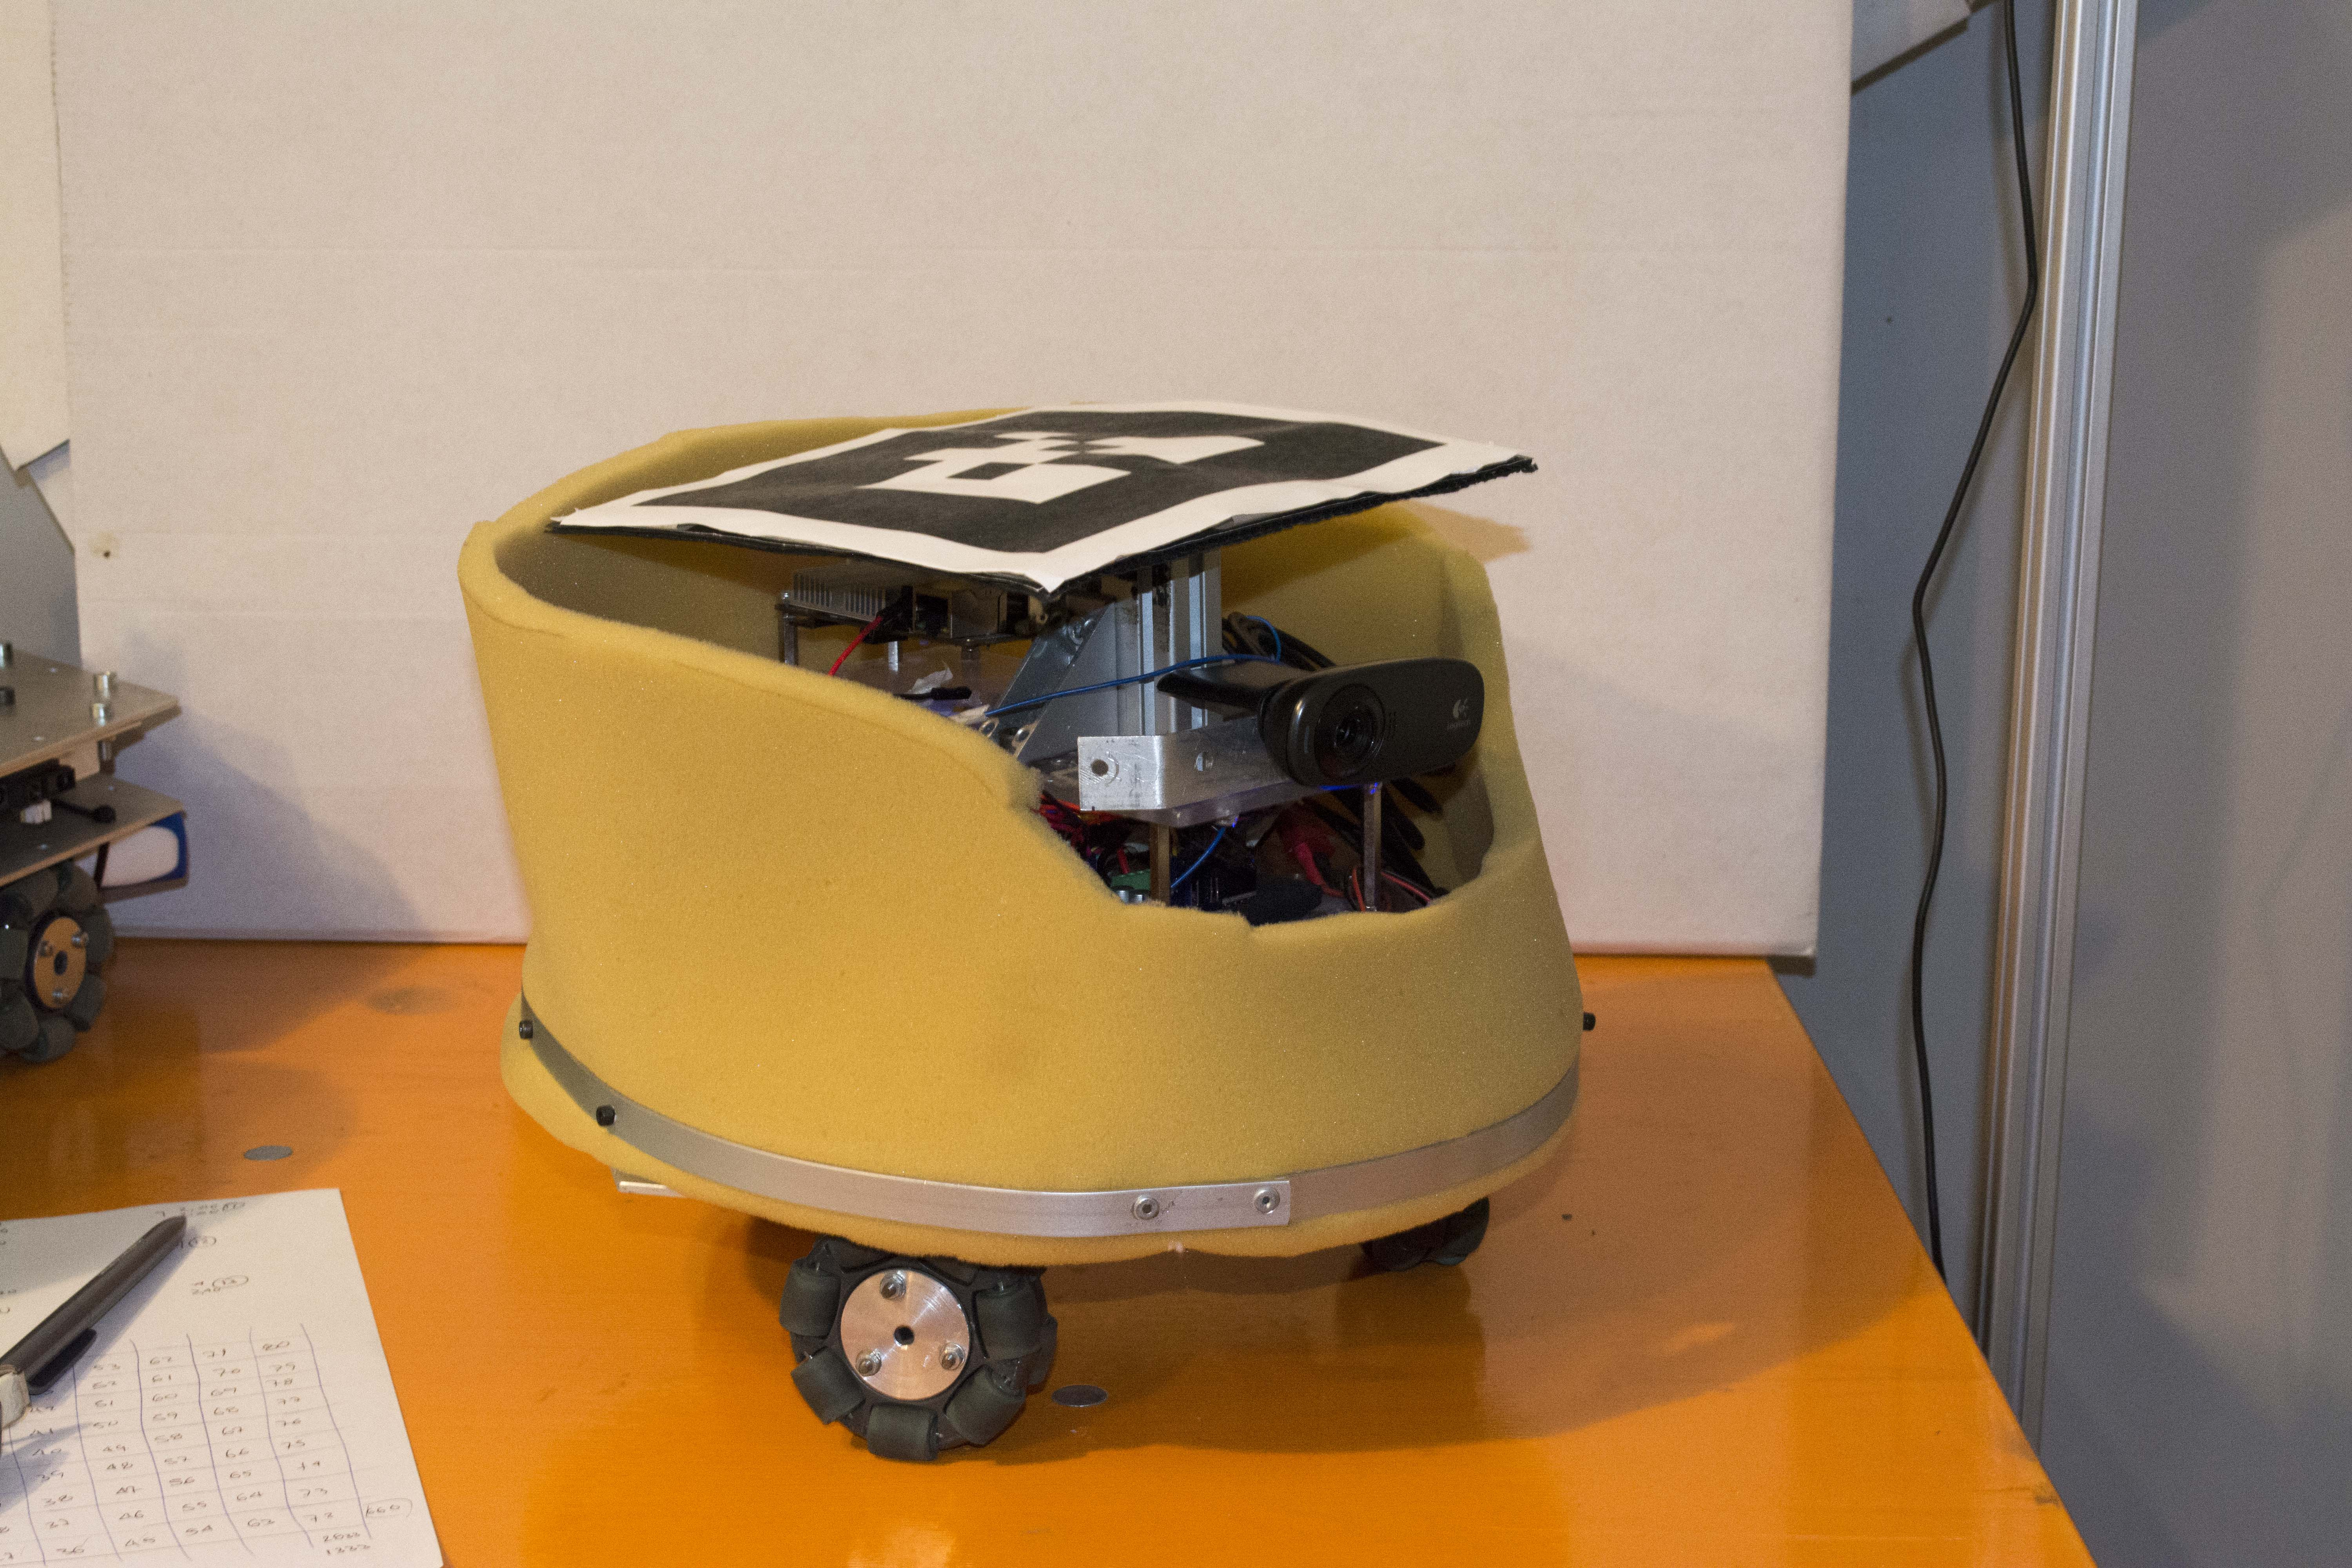
\includegraphics[height=3cm]{./Images/DSC_0447.JPG}}
\hspace{2mm}
\subfigure{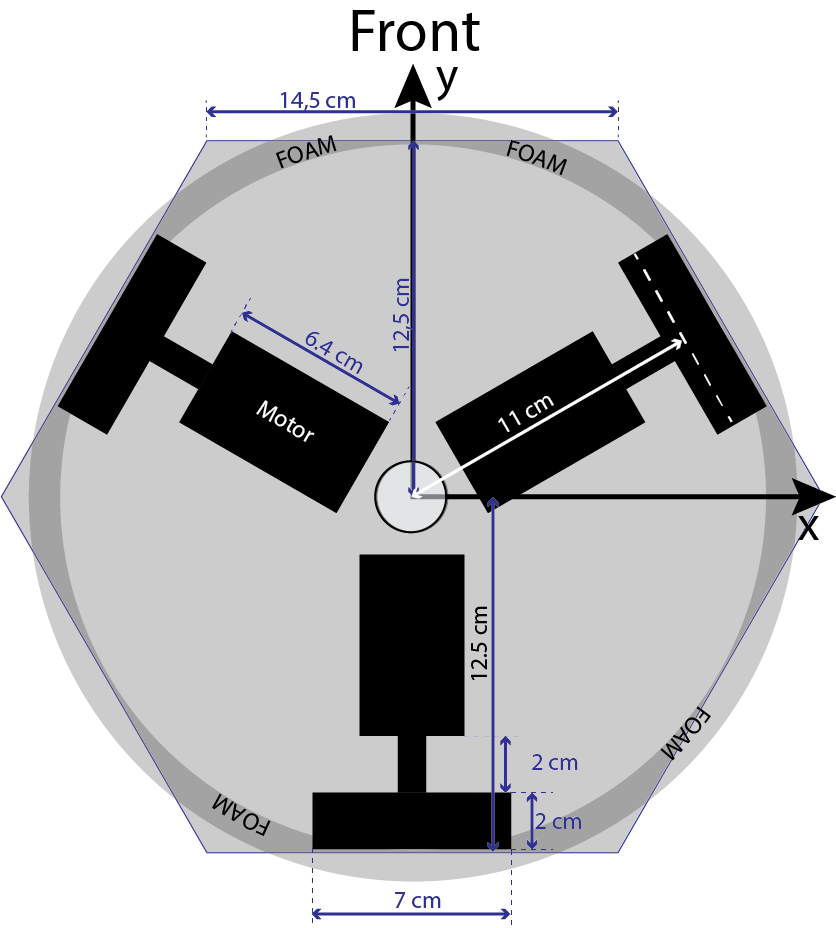
\includegraphics[height=3cm]{./Images/TriskarThird.png}}
\caption{Platform used in the case study (left), and holonomics's blue prints (right). The arrows represent robot's frame of reference.
\label{fig:Robot}}
\end{figure}

\subsection{Emotion Enrichment System}

The main idea of Emotional Enrichment System is to blend an emotion and a action to generate the effect of "emotional action". However this is not far as previous works have done so far. Therefore, the system has been envisioned to also enable:

\begin{itemize}
	\item Interoperability among different platform.
	\item Introduction of new parameters and emotions.
	\item Interface with diverse action decision system.
\end{itemize}

In other words, the system could be thought as a black box that receives a desire action, action's parameters and emotion to blend them together without paying particular attention on who or how the decision to execute a particular action was made. This is achieved through the use of messages to describe the action that should be executed, as well its parameters, emotion and emotion's intensity.  These information are divided into two messages: one for the action and its parameters, and other for the emotion and its intensity. This is done to do not affect the action's execution.

Every time the system receives a new action, it verifies if the action exists and parameters corresponds to the desire action. If these two conditions are met, then the system checks if the action is compound or simple. If it is a simple, the system proceeds to add all the required actions (emotional actions) and change their parameters to convey the desired emotion. On the other hand if the action is compound, the action is first decomposed in simple actions (mandatory actions). Each one of these actions is then process to add their emotional actions. However, this addition is done taking in consideration to not add any action that was previously added. Once all the set of simple actions and their parameters are determined, the system proceeds to verify the drivers' existence to execute these actions in the desired platform. If the system finds out that one or more mandatory actions could not be executed, it triggers a message to inform that the desire action could not be executed. 

%%%%%%%%%%%%%%%%%%%%%%%%%%%%%%%%%%%
\subsubsection{Simple and Compound Actions}

To achieve actions' enrichment with emotions, two different types of actions are used: simple and compound actions. Simple actions are actions that could be considered as ''atomic''; these actions can be enriched with emotion changing their specific parameters. For example, consider two simple actions: speak and move body. The human action of speaking is related to changes in the vocal cords to produce different sounds, while move body is directly related to the body movement. Therefore, for the speaking action the following parameters are expected: text, pitch and tone. On the other hand, the action move body would have as parameters the desired destination, velocity, and trajectory constraints. Since each action is characterized by different parameters, parameters' modifications to obtain an emotional action will be different for each of them. On the other hand, compound action is an action created from other compound or simple actions. For example, suppose that it is required that the robot has to \textit{recite} some dialogue and \textit{walk} to a different positions, as doing a trajectory. A possible implementation could consist on speak simple action in parallel to two consecutive action walk, which is also a compound action that is composed by three parallel actions: balance left arm, balance right arm, and move body.

Although compound actions could be used to generate diversity of actions from simple actions, the main drawback of this approach is that all possible combination of actions should code in the system to be used. Using the example previously described, if it is decided to have three positions instead of two, then it would mean that a new compound action should be implemented to have an action in which could be specified three positions. To overcome this limitation, it was created a language to specify actions that are not implemented in the system. A computational representation of these language is used to execute the actions described in this language. 

\subsubsection{Emotional Execution Tree}
The \textit{Emotional Enrichment System}  is grounded on the use of \textit{Emotional Execution Tree} ($EXT$), which is a computational representation of desired actions that must be executed. 
$EXT$ is a connected acyclic graph with vertices and  edges. The root and non-leaf nodes could be \textit{parallel} or \textit{sequence} type. The parallel node could be one out of four different sub-types: action and emotion synchronous, action synchronous and emotion asynchronous, action asynchronous and emotion synchronous, or action and emotion asynchronous. Sequential nodes could just be one of two sub-types: emotion synchronous or asynchronous. Action synchronous means that each time that a parallel node receives a finish notification (success or failure), it will send a finish message to all the nodes that derived from it. On the other hand, emotion synchronous means that each time that a node (sequence or parallel) receives an emotion synchronization message, it will propagate the message to all the actions in the branches. 
This distinction creates the possibility to synchronize emotional changes without affecting the normal execution of the desired action. Finally, the leaf nodes could only be simple action nodes. All the nodes can assume two levels: principal or secondary. If a node is principal, it will notify its predecessor about the messages that it has received, while the secondary cannot propagate any message to its predecessor.

\subsubsection{Implementation}
Figure~\ref{fig:system_architecture} presents the design used to achieve the desire goals. As it could be observed, the system is divided in two parts. The first part in charge to enrich a given action with a desired emotion, and the second in charge to hide the real execution of the action. 

\begin{figure*}
	\centering
	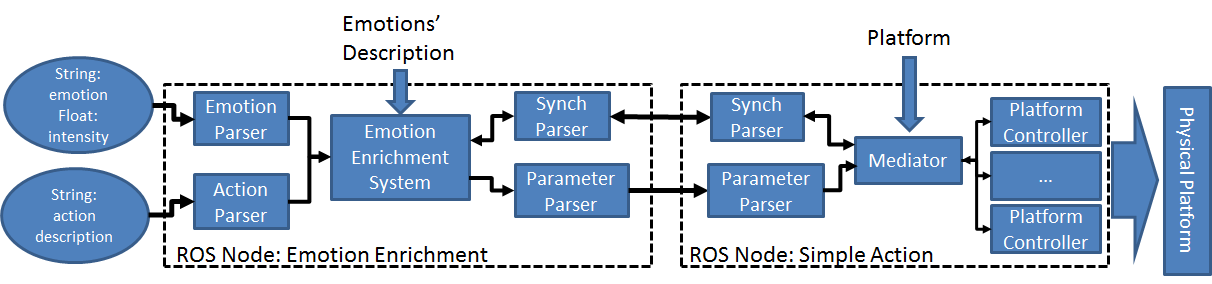
\includegraphics[width=1.0\textwidth]{Images/SystemArchitecture.png} 	
	\caption{General system design. Each simple action corresponds to one ROS node, and there is just one node for the emotion enrichment system. The ovals represent the ROS topic parameters, rectangles represent \textit{black boxes}, and texts outside containers represent input files that contain the system parametrization.}
	\label{fig:system_architecture}
\end{figure*}

The action enrichment is achieved through the following phases:
\begin{enumerate}

	\item \textit{Generation of emotional execution tree:} this phase starts every time that a new action message is received. The process begins by parsing the format, verifying that the actions described on it exist in the system, and that the parameters correspond to the ones expected by each action described in the message. This parameters' verification is done on the implemented description for each simple action, which describes the parameters that are mandatory and those that are optional. When the verification is done, and all the action exists and  the parameters correspond, an $EXT$ is created.

	\item \textit{Emotion addition:} uses the $EXT$ created in the previous phase. In this phase new simple actions are added to the $EXT$ and the simple action's parameters are modified following emotions' descriptors, which are loaded from files. This process is broken down in two steps. First, all actions that are required to convey the desired emotion, and that are not yet present in the branch are added. Second, the emotional parameters are modulated based on the emotion's intensity and character traits.

	\item \textit{Execution:} this is the last phase and it is done after the $EXT$ is ''coloured'' with emotional characteristics (actions additions and emotional parameters). The decision to have two different communication channels, one for action parameters and another for the action emotional parameters, was taken to enable the possibility to update the emotional parameters without interfering with the current execution. In this phase is maintain a reference to the mandatory and emotional action, thus when a new emotion is received the system stops the previous emotional action and start executing the new ones without affecting the general execution of the actions.

\end{enumerate}
\section{Case Study}
\label{sec:case}
 The case study presented in this paper was held at an exhibition with two main objectives:
\begin{enumerate}
	\item Cross-validate the findings obtained from a previous experiment~\cite{Angel2017-2}. This experiment was done to study the attribution of different linear and angular velocities, oscillation angle, direction, and orientation of the platform to \textit{Anger}, \textit{Happiness}, \textit{Sadness} and \textit{Fear}. A total of 196 value combinations were designed, 20 of which were presented to each participant. Subjects had to select for each presentation the most representative term describing it among the four emotions and two mental states (i.e., \textit{Excitement} and \textit{Tenderness}).
	\item Verify whether participants would prefer scenes when the robot moves expressing emotions or rather moves on the same trajectory without any emotion expression. To control scene variability two cameras and eight AR tags were used together with a Kalman filter to improve robot localization on the stage. AR tags were detected using the ROS package ar\_track\_alvar~\cite{artag2015}. The distribution of thecameras and the tags is reported in Figure~\ref{fig:setup_fourth}. 

\begin{figure}
	\centering
	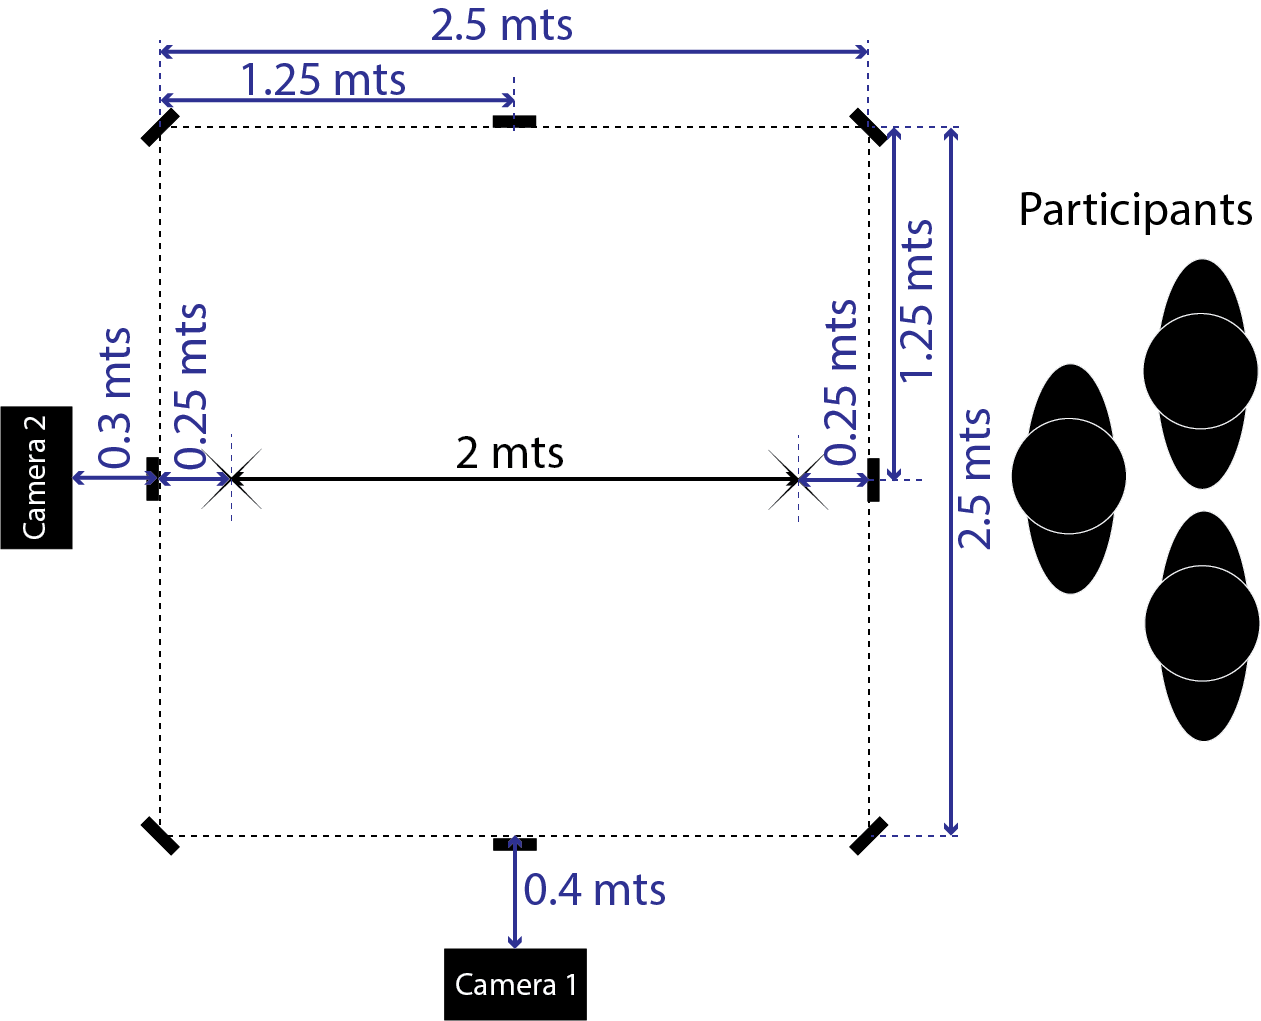
\includegraphics[width=0.45\textwidth]{./Images/FourthCase.png} 
	\caption{Environment setup for the case study. The crosses represent the starting points.}
	\label{fig:setup_fourth}
\end{figure}
 
\end{enumerate}

\subsection{Emotion Description}

The parameters selected to implement \textit{Anger}, \textit{Happiness}, \textit{Sadness} and \textit{Fear} are shown in Table~\ref{table:selected_fourth}. As it could be observed, two configurations for each emotion were selected among the ones evaluated in the previous experiment to be cross-checked. These configurations had to satisfy two conditions: (i) the linear velocity should be greater than $0$, so the robot should show some displacement, and (ii) it should be in the top 10 list of the configurations tested in the previous experiment.

\begin{table}
\centering
\small
\caption{Parameter values selected from the previous experiment.}
		\label{table:selected_fourth}
		\begin{tabular}{|c|p{0.9 cm}|p{0.9 cm}|p{0.9 cm}|p{1.05 cm}|p{0.9 cm}|}
			\hline
%\rotatebox{90}{\textbf{Emotion } }&
%\rotatebox{90}{\textbf{Direction  ($rad$)}}&
%\rotatebox{90}{\textbf{Orientation ($rad$)} }&
%\rotatebox{90}{\textbf{Linear Velocity ($mm/s$) }}&
%\rotatebox{90}{\textbf{Angular Velocity ($rad/s$) }}&
%\rotatebox{90}{\textbf{Angle ($rad$)}}\\	
\textbf{Emotion}&\textbf{Direc-tion  ($rad$)} & \textbf{Orien-tation ($rad$)} & \textbf{Linear Velocity ($mm/s$) } & \textbf{Angular Velocity ($rad/s$) } & \textbf{Angle ($rad$)} \\
			\hline
			Happiness-1&$0$&$0$&$500$&$3$&$0.349$\\
			\hline
			\co Happiness-2&\co $0$&\co $0$&\co $900$&\co $3$&\co $0.174$\\
			\hline
			Anger-1&$\pi$&$0$&$500$&$3$&$0.087$\\
			\hline
			\co Anger-2&\co $0$&\co $0$&\co $900$&\co $1$&\co $0.087$\\
			\hline
			Fear-1&$\pi$&$\pi$&$900$&$2$&$0.174$\\
			\hline
			\co Fear-2&\co $\pi$&\co $\pi$&\co $500$&\co $2$&\co $0.087$\\
			\hline
			Sadness-1&$\pi$&$0$&$200$&$1$&$0.349$\\
			\hline
			\co Sadness-2&\co $0$&\co $\pi$&\co $200$&\co $1$&\co $0.349$\\
			\hline
			\end{tabular}
\end{table}


\subsection{Scene}

Stage discretization was used to give zones of movements instead of absolute positions. This idea was brought from human theatrical actors, who arrange their movements based on zones on the stage~\cite{wilson2009theatre}. This allows them to adapt their position based on other actors and stage dimensions. The stage was discretized in 9x9 matrix as shown in Figure~\ref{fig:stage_division}. Robot's movements are given in terms of matrix positions to the Emotional Enrichment System. The robot's final position is calculated by the Emotional Enrichment System during execution. For instance, the scene was designedon a 3 x 3 meters stage, but in the presentation at teh exhibition the stage was 2.5 x 2.5 meters.

\begin{figure}
	\centering
	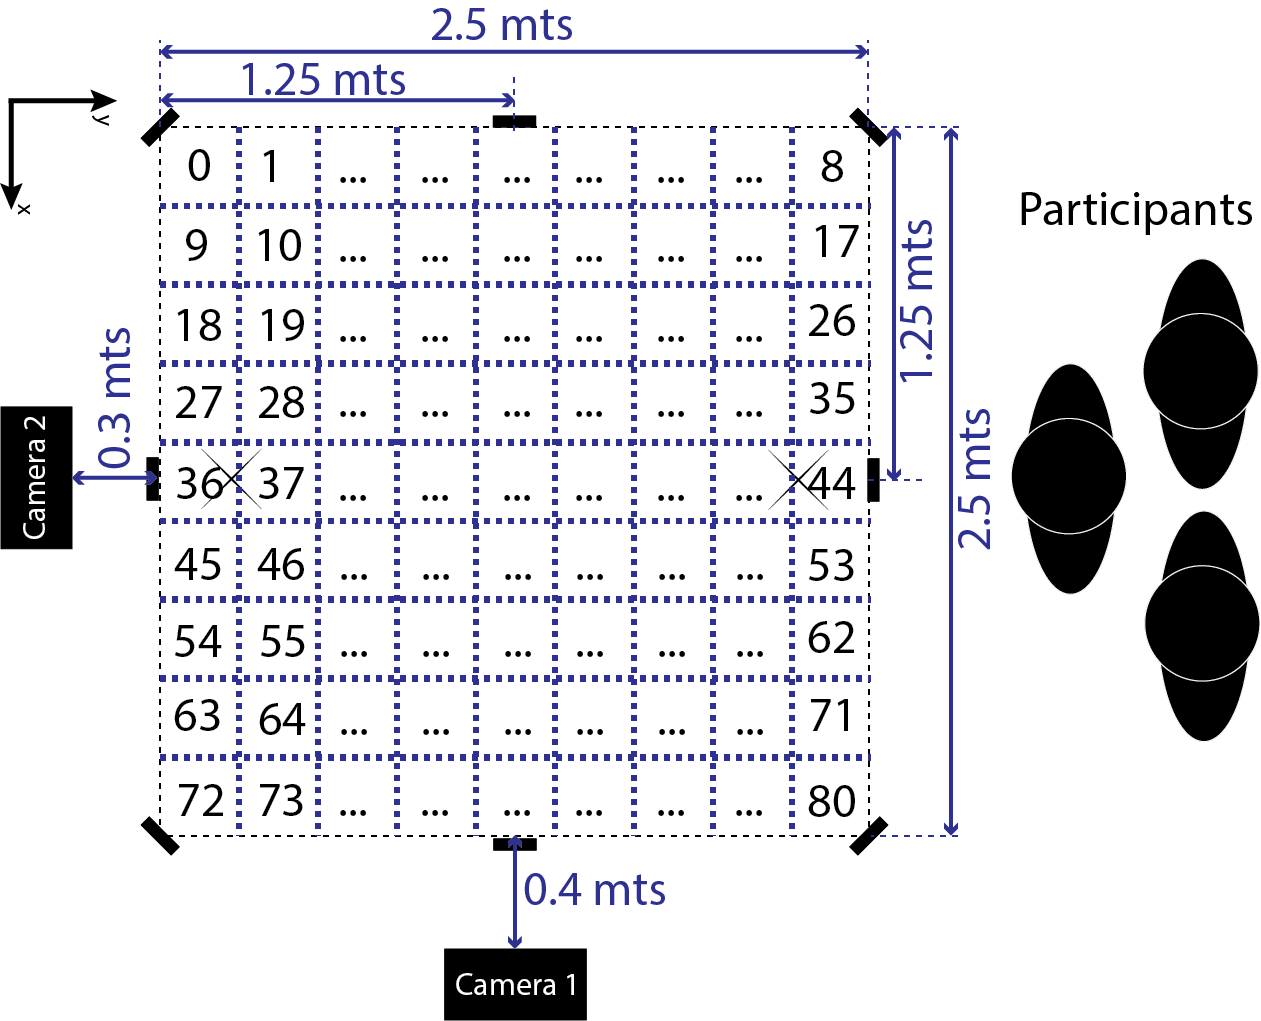
\includegraphics[width=0.45\textwidth]{./Images/FourthCaseScene.png} 
	\caption{Stage discretization  used for the scene. The blue squares correspond to the each zone, while the numbers correspond to the ID given to each zone.}
	\label{fig:stage_division}
\end{figure} 

The scene can be described as follows. The robot starts in the middle of the stage to move to the upstage right (See~\cite{Musical}), close to the right wing. Then, the robot moves to upstage right center and rotates to $\pi/2$ left (See~\cite{Artopia}). Next the robot moves to the right center. Then it goes to the center. When it arrives there, it turns full back and move backwards to downstage center with a full front orientation. There, it turns full back to move to center. Finally the robot turns to profile right and it does a step back; then it goes to the upstage center and then upstage right. The sequence of movements programmed to the robot are depicted in Figure~\ref{fig:movement}.
\begin{figure*}
	\centering
	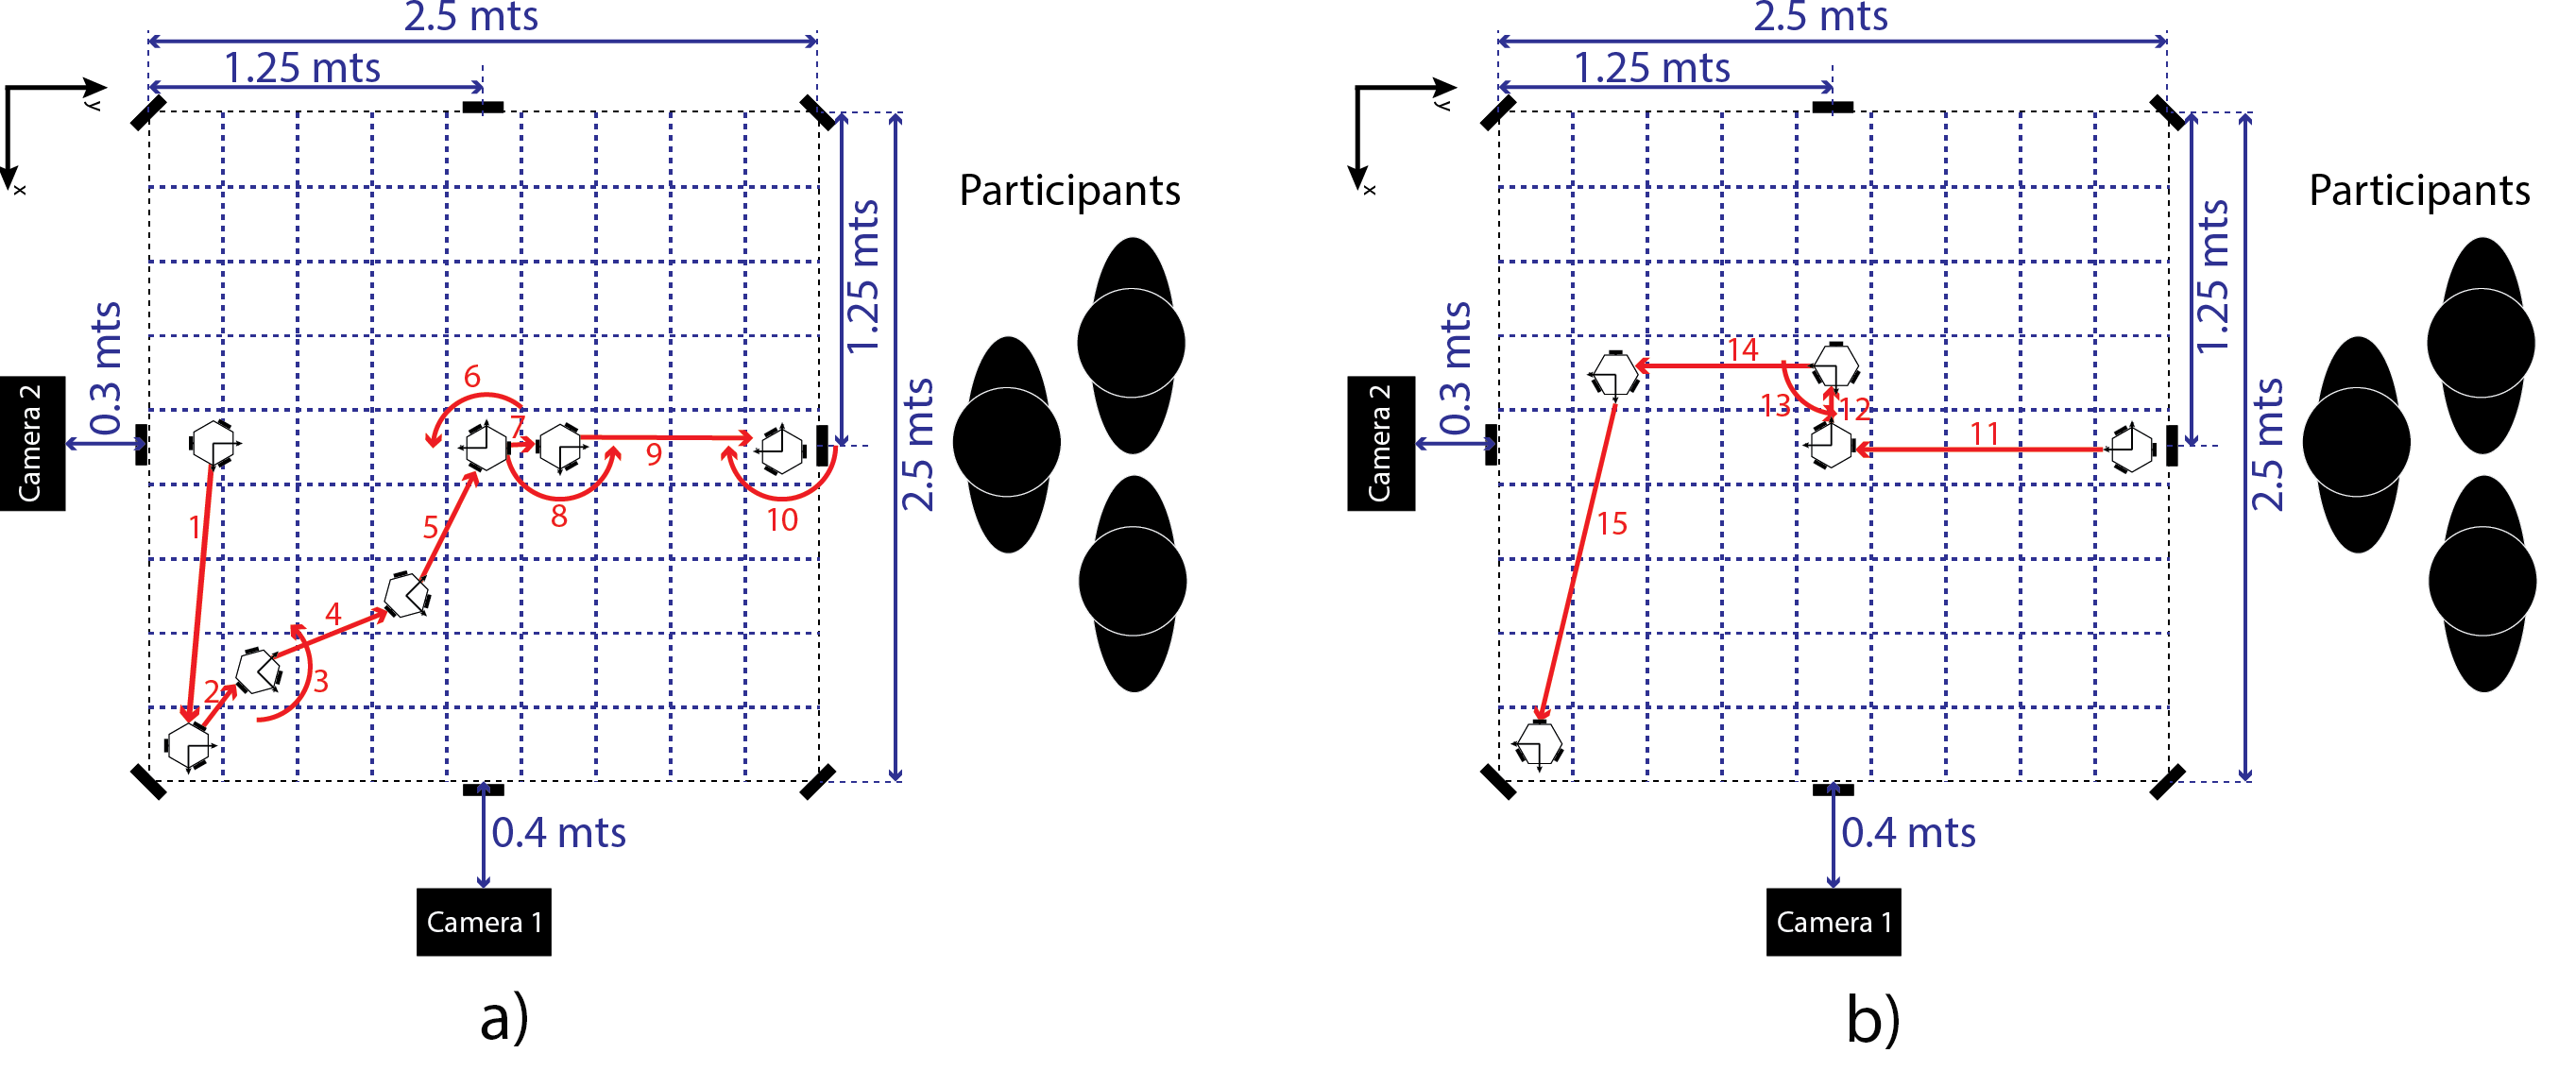
\includegraphics[width=0.95\textwidth]{./Images/fourthCaseSceneD.png} 
	\caption{Sequence of movements provided to the robot. The red arrows show the trajectory, while the numbers show the order among the movements. a) The first ten movements b) The last five movements }
	\label{fig:movement}
\end{figure*}

The relation between emotion and movement is as follow: movements one to five do not express any emotion. Movements six to ten show fear. Movement eleven depicts happiness, and the remaining movements depict sadness. The actions describing this scene are executed by the Emotional Enrichment System and the emotion selection is done manually via a graphical interface.

\subsection{Study}

This case study was done during Researchers' Night, 2015. During a period of two days, people were asked to participate in this study, which was divided in to parts. The first one, each subject was exposed to two rounds of emotions. The two emotions and their other were generated randomly before hand. The second part, participants were explained that a small scene was going to be presented twice. Thus, they should to selected the one they like more. The order of the scenes (e.g. with or without emotion) were generated beforehand. The total number of volunteers was 256: 128 males, 126 females, and 2 that chose not to specify their gender. The average age was 27.29 years, with standard deviation of 16.58, minimum age was 4 and maximum 76.

\section{Results}
\label{sec:results}
This section reports the results obtained during two days for the two parts of the case study.

\subsection{Part I: Emotion Recognition}

The results obtained from the presentation of emotional movements are summarized in 
Table~\ref{table:result_fourth}. 
\begin{table}
\centering
\small
\caption{Summary of the answers obtained in the presentation of emotional movements.}
		\label{table:result_fourth}
		\begin{tabular}{|c|c|c|c|c|c|c|c|c|}
			\hline
\rotatebox{90}{\textbf{Presented/Reported } }&
\rotatebox{90}{\textbf{Happiness}}&
\rotatebox{90}{ \textbf{Anger}} &
\rotatebox{90}{\textbf{Fear}}&
\rotatebox{90}{\textbf{Sadness}}&
\rotatebox{90}{\textbf{Excitement}}&
\rotatebox{90}{\textbf{Tenderness}}&
\rotatebox{90}{\textbf{Other}}&
\rotatebox{90}{\textbf{Total}}\\	
			\hline
			Happiness-1&8&16&7&4&16&4&7&62\\
			\hline
			\co Happiness-2&\co 11&\co 11&\co 6&\co 2&\co 19&\co 3&\co 1&\co 53\\
			\hline
			Anger-1&7&5&6&2&21&7&1&49\\
			\hline
			\co Anger-2&\co 14&\co 29&\co 13&\co 2&\co 13&\co 3&\co 2&\co 76\\
			\hline
			Fear-1&6&2&28&1&9&6&0&52\\
			\hline
			\co Fear-2&\co 7&\co 3&\co 37&\co 2&\co 20&\co 4&\co 1&\co 74\\
			\hline
			Sadness-1&3&5&17&14&5&16&5&65\\
			\hline
			\co Sadness-2&\co 5&\co 5&\co 15&\co 28&\co 6&\co 15&\co 7&\co 81\\
			\hline
			\end{tabular}
\end{table}

It could be observed that both implementations of \textit{Happiness} were confused with \textit{Anger} and \textit{Excitement}. In a similar way, Anger-1 was mostly confused with \textit{Excitement}, which was voted twenty one over forty nine subjects.
Anger-2 shows an improvement of perception from 10\% to 38\%, respect Anger-1. This implementation was perceived also as \textit{Happiness}, \textit{Fear} and \textit{Excitement}.
Both implementations of \textit{Fear} had a high level of recognition 54 \% and 50 \% and mostly confused with \textit{Excitement}, which was voted nine times for the first implementation and twenty times for the second implementation. Finally, the two implementation of \textit{Sadness} were confused with \textit{Fear} and \textit{Tenderness}.

An analysis was done per groups, for each presented emotion. For each emotion it was considered how many subjects in each group recognized it, how many identified a different emotion, how many identified the considered emotion when presented another one, and how many subjects recognized an emotion different from the considered one when presented a different emotion. This lead to a table, which is known as contingency table, for each presented emotion, like the one reported in table~\ref{table:singleEmotion} for Happiness-1. 
\begin{table}[!htbp]
\begin{center}
\caption{Example of table compiled for each emotion on the subjects which have been presented each emotion (here Happiness-1).}
\label{table:singleEmotion}
\begin{tabular}{|c|c|c|}
\hline 
Presented/Reported&Happiness&Other\\
\hline 
Happiness-1&8&54\\
\hline 
Other&42&355\\
\hline
\end{tabular}
\end{center}
%\vspace{-0.5cm}
\end{table}

For each of the contingency table the classification accuracy and the no-information rate (NIR), i.e. the accuracy that had been obtained by random selection, are reported in Table~\ref{table:nir_fourth}. The results reveal that Sadness-2 is the only implementation that was correctly recognized among all implementations ($p<0.05$). 

\begin{table}
\centering
\small
		\caption{Classification accuracy of the presented emotions by the single panels, computed as mentioned in the text, with corresponding 95\% confidence interval, no-information rate, and p-value that accuracy is greater than the NIR.}		
		\label{table:nir_fourth}
			\begin{tabular}{|p{1.8 cm}|c|c|c|c|}
				\hline		
\rotatebox{90}{\textbf{Presented Emotion}}&
\rotatebox{90}{\textbf{Classification Accuracy}}&
\rotatebox{90}{\textbf{95\% CI}}&
\rotatebox{90}{\textbf{No-Information Rate}}&
\rotatebox{90}{\textbf{P-Value [Acc $>$ NIR]}}\\
				\hline
			Happiness-1&0.79&(0.75,0.82)&0.89&1.0\\
			\hline
			\co Happiness-2&\co 0.81&\co (0.77,0.84)&\co 0.88&\co 1.0\\
			\hline
			Anger-1&0.8&(0.76,0.83)&0.88&1.0\\
			\hline
			\co Anger-2&\co 0.89&\co (0.76,0.84)&\co 0.83&\co 0.95\\
			\hline
			Fear-1&0.79&(0.75,0.83)&0.88&1\\
			\hline
			\co Fear-2&\co 0.78&\co (0.73,0.81)&\co 0.83&\co 0.99\\
			\hline
			Sadness-1&0.85&(0.81,0.88)&0.84&0.47\\
			\hline
			\co Sadness-2&\co 0.85&\co (0.81,0.88)&\co 0.81&\co 0.035\\
			\hline
			\end{tabular}
\end{table}

Additionally, the positive predictive value, accuracy and a Pearson's $\chi^2$ were computed for each table. The hypothesis used in the test were:

\begin{itemize}
	\item $H_0 = $ there is a difference in recognition between the implementation respect the others.
	\item $H_1 = $ there is not a difference in recognition between one implementation respect the others.
\end{itemize} 

The results are shown in table~\ref{table:Precision2}. They show that there is significant evidence to conclude that Anger-2, both of \textit{Fear} and \textit{Sadness} are considered as a different implementation when they are compare with other implementations. While both implementations of \textit{Happiness} and Anger-1 are considered as similar to the other implementations. 

\begin{table}
\centering
\small
\caption{Accuracy, precision and results of Pearson's $\chi^2$ for each contingency matrix with $\alpha = 0.05$ for the case study.} 
\label{table:Precision2}
		\begin{tabular}{|p{1.6 cm}|p{1.5 cm}|c|c|c|}
		\hline
		\textbf{Presented Emotion} & \textbf{Positive Predicted Value} & \textbf{Accuracy} & \textbf{$\chi^2(1)$} & \textbf{p-value}\\
		\hline
		Happiness-1 & $0.13$ & $0.79$ & $0.11$ & $0.74$\\
		\hline
		\co Happiness-2 &\co $0.21$ &\co $0.81$ &\co $3.7$ &\co$0.054$\\
		\hline
		Anger-1 & $0.1$ & $0.8$ & $3.8e^{-29}$ & $1$\\
		\hline
		\co Anger-2 &\co $0.38$ &\co $0.81$ &\co $34.4$ &\co $<0.001$ 
		%4.47e-9
		\\
		\hline
		Fear-1 & $0.54$ & $0.8$ & $36.2$ & $<0.001$ 
		%1.8-e9
		\\
		\hline 
		\co Fear-2 &\co $0.5$ &\co $0.78$ &\co $35.8$ &\co $<0.001$ 
		%5.3e-10
		\\
		\hline
		Sadness-1 & $0.22$ & $0.85$ & $27.4$ & $<0.001$
		%$1.63e-7$
		\\
		\hline
		\co Sadness-2 &\co 0.35 &\co 0.85 &\co 72.9 &\co $<0.001$
		%2.2e-16
		\\		 
		\hline
			\end{tabular}
\end{table}  

To determine if which implementations were perceived as different or similar, a Fisher's exact test was applied for ten different combinations of the implementations. Additionally, a Holm-Bonferroni correction was applied for multiple comparisons to get a better p-value estimation. The following are the hypothesis used in this test:

\begin{itemize}
	\item $H_0 = $ there is a difference in the recognition of the two compared emotions.
	\item $H_1 = $ there is not a difference in the recognition of the two compared emotions.
\end{itemize}

The results are reported in Table~\ref{table:result_compare_fourth}. As it could be observed, both implementation of \textit{Anger} were perceived as two different emotions ($p<0.001$). Also shows that both implementation of \textit{Happiness} were perceived as to Anger-2 ($p=0.69$ in both cases).

\begin{table}
\centering
\small
\caption{Pair comparison among all the implemented emotions using Fisher's exact test for both questionnaires with $\alpha = 0.05$ for the  case study. The * indicates that the p-value was adjusted using the Holm-Bonferroni correction for multiple comparisons.}
		\label{table:result_compare_fourth}
		\begin{tabular}{|c|c|c|}
			\hline	
\textbf{Pair Compared} & \textbf{p-value} & \textbf{p-value*}\\	
			\hline
			Happiness-1 vs Happiness-2 &$0.38$&$1.0$\\
			\hline
			Anger-1 vs Anger-2 & $<0.001$ 
			%7.3e-4
			& $<0.001$
			%4.4e-3
			\\
			\hline
			Anger-2 vs Happiness-1 & $0.137$&$0.69$\\
			\hline
			Anger-2 vs Happiness-2 & $0.157$&$0.69$\\
			\hline
			Fear-1 vs Fear-2 & $0.74$&$1.0$\\
			\hline
			Sadness-1 vs Sadness-2 & $0.665$&$1.0$\\
			\hline
			Fear-1 vs Sadness-1& $<0.001$ 
			%8.35e-5
			& $<0.001$
			%5.8e-4
			\\
			\hline
			Fear-1 vs Sadness-2 & $<0.001$
			%5e-7
			& $<0.001$
			%4e-6
			\\
			\hline
			Fear-2 vs Sadness-1 & $<0.001$
			%2e-7
			& $<0.001$
			%1.8e-6
			\\
			\hline
			Fear-2 vs Sadness-2 & $<0.001$
			%1e-7
			& $<0.001$
			%1e-6
			\\
			\hline
			\end{tabular}
\end{table}  
 
Nevertheless, it is important no notice that the results were obtained using the lower part of the robot without any change in shape. Another important factor to highlight is the impact words listed in the questionnaire have on the perception rate. As it was expected, mental states Excitement and Tenderness were confused with emotions with similar arousal level. In this precise case the emotions Anger, Happiness and Fear were confused with Excitement, and Sadness was confused with Tenderness. Despite the bias generated by the two mental states listed in the questionnaire, the recognition rate of five out of eight implementations was over 35\%, being the two implementation of \textit{Fear} the implementations with the higher recognition rates (54\% for the first and 50\% for the second).

\subsection{Part II: Scene Preference}

The results obtained form the small scene are presented in Table~\ref{table:preference_selection}. From this data, two questions wanted to be answer:
\begin{enumerate}
	\item Do people prefer scenes with or without emotions?
	\item Has gender an impact in the preference?
\end{enumerate}
To answer these questions the following hypothesis were created:
\begin{enumerate}
	\item $H_0 =$ there is a preference towards scenes with emotions. $H_1$ there is a preference towards scenes without emotions. 
	\item $H_0 =$ there is an association between gender and the preference. $H_1 =$ there is not an association between gender and the preference. 
\end{enumerate}
A $\chi^2$ test with one degree of freedom and $\alpha = 0.05$ was done to verify them. The results of the tests show that there is enough statistical evidence to accept that people prefer scenes with emotions ($p<0.001$). On the other hand, the test shows that there is not association between gender and preference $(p=0.85)$.

\begin{table}
\centering
		\caption{Answers obtained for the small scene.}		
		\label{table:preference_selection}
			\begin{tabular}{|c|c|c|c|}
			\hline
			\textbf{Gender}&\textbf{With Emotion}&\textbf{Without Emotion}&\textbf{Total}\\
			\hline
			Male & 84 & 43 & 127\\
			\hline
			Female & 81 & 45 & 126\\
			\hline
			\textbf{Total} & 165 & 88 & 253\\
			\hline
			\end{tabular}
\end{table}

\section{Conclusions and Further work}
The case study presented in this paper was done to cross validate the findings in the experiment and verify whether the participants would prefer scenes when the robot expresses emotions or rather moves without any emotion expression. For each one of four emotions (i.e. Anger, Happiness, Sadness and Fear) studied in the experiment were selected a two set of parameters.The results show that both implementations of happiness were confused with anger and excitement, while one implementation of anger was just confused with excitement. Both implementations of sadness were confused with tenderness and fear. Both implementations of fear had a recognition rate over 50\%. Scenes results show that people prefer scenes with emotional movements and there is not any difference in gender.

Additionally to the results already mentioned, there are words that could bias participants' perception. For instance happiness and anger were considered as excitement. This misinterpretation should not be a surprise given the fact that there is not a unique definition of emotion~\cite{Plutchik2001,cacioppo2000handbook}, and each person would interpret a situation differently, so they will give a different label to the presented movement. Moreover a misinterpretation of Happiness and Anger could suggest that additional features (e.g. trajectory or shape) should be added to increase differentiation between these two emotions. For example, Venture and collaborators~\cite{Venture2014} had found out that in human bodies the recognition rate of anger and fear are increased when torso and head are downwards. On the other hand, they found that happiness perception is increased when the torso and head are move upwards. This example could bring some insight to possible body changes that could occur in non-human like bodies, but it should tested in this kind of platforms to confirm if the same impact is reached.
 
\break
\bibliographystyle{splncs}
\bibliography{Bibliography,BibloNew,Biblography}
\end{document}
